\documentclass[a4paper]{article}
\usepackage{graphicx}

\title{Architecture of a multi agent approach for a bakery}
\author{Angela Enriquez\\
	    Ethan Massey\\
	    Erick Kramer}

\begin{document}
	\maketitle
	\newpage
	\section{Architecture pipeline}
	
	\begin{figure}[h!]
		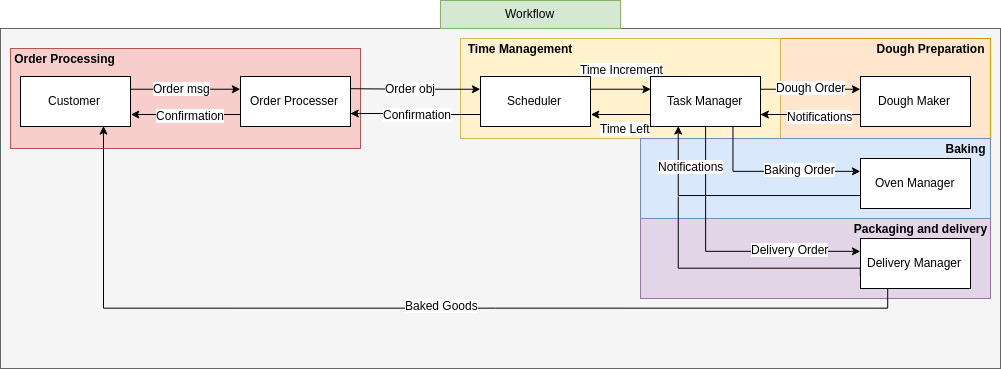
\includegraphics[scale=0.4]{img/architecture-pipeline.png}
		\caption{Pipeline of the architecture.}
	\end{figure}
	
	\section{Agents}
	
	\begin{figure}[h!]
		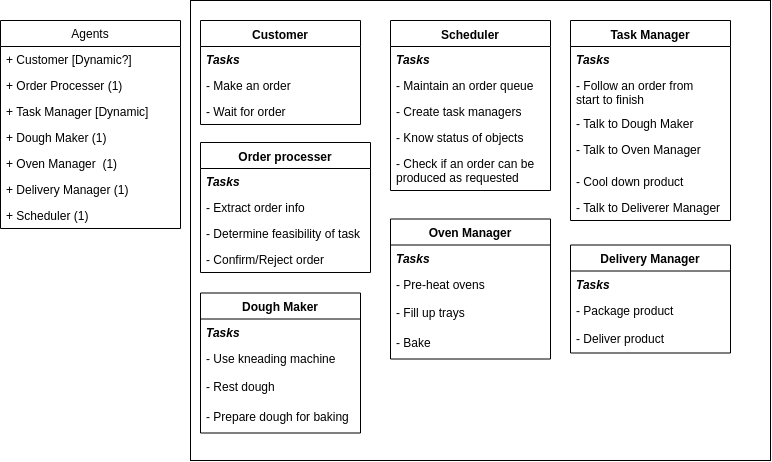
\includegraphics[scale=0.5]{img/architecture-Agents.png}
		\caption{Agents that conforms the system.}
	\end{figure}
	\newpage
	\section{Objects}
	
	\begin{figure}[h!]
		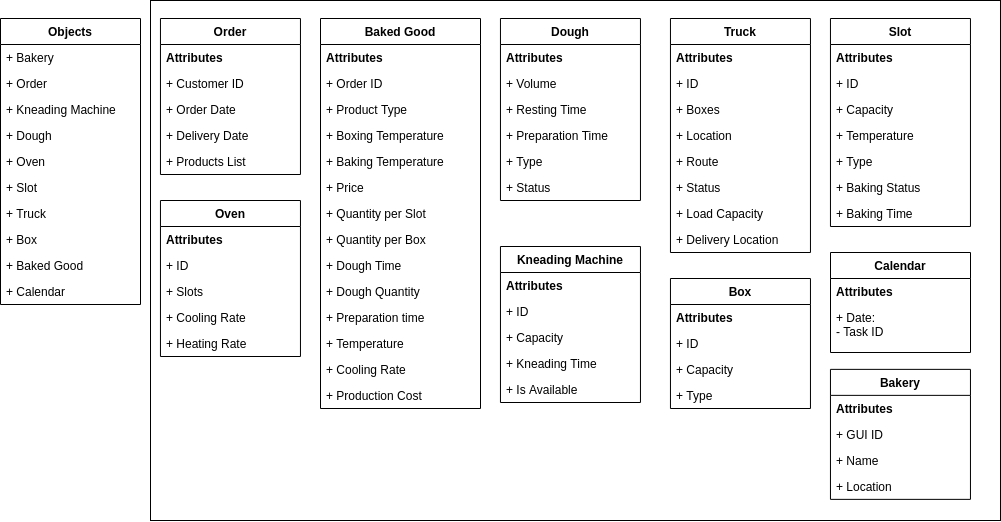
\includegraphics[scale=0.4]{img/architecture-Objects.png}
		\caption{Objects used in the system.}
	\end{figure}
	
	The scheduler agent is going to be the responsible for the orders received from the customers. 
\end{document}